\documentclass{article}
% Language setting
\usepackage[english]{babel}

% Set page size and margins
\usepackage[a4paper]{geometry}

% Useful packages
\usepackage{amsmath}
\usepackage{graphicx}
\usepackage[colorlinks=true, allcolors=blue]{hyperref}

% images
\usepackage{graphicx}
\graphicspath{ {./images/} }

\renewcommand*\contentsname{Summary}

\title{%
  JavaScript Security: Theory and Practice \\
  \large Cryptography Course Paper and Project (Prof. S. Cimato)}
\author{Sergio Meloni, 773779 - February 2024}
\date{\vspace{-5ex}}
%\date{}  % Toggle commenting to test

\begin{document}
\maketitle

{
 \hypersetup{linkcolor=black}
 \tableofcontents
}

\iffalse
Intro lunga
JavaScript and Security
- History
- Security
JavaScript Threats
- XSS
Project
- Introduction
- Source Code (?)
\fi

\newpage
\maketitle
\section{Introduction}

JavaScript has become one of the most important pillars of modern web development. Originally created to add interactivity to web pages, over the years it has evolved from a simple tool for automating minor actions in browsers to a powerful and flexible programming language capable of handling complex and high-performance web applications. Its versatility extends over the confines of the browser, finding applications on the server side, in mobile app development, game programming, and even in areas such as IoT (Internet of Things).
\\
\\
One of the most attractive aspects of JavaScript is its \textbf{accessibility}: with a relatively easy learning curve, it is often the first language that new developers approach. This ease of use, combined with a vast and active community that contributes an infinity of frameworks, libraries, and tools, makes JavaScript particularly welcoming for those beginning their journey into the world of programming.
\\
\\
However, the simplicity of JavaScript bring significant \textbf{security challenges}. The open nature of the web and the interoperability between various systems and technologies expose JavaScript applications to a wide range of vulnerabilities and cyberattacks. Common programming errors, such as failing to sanitize user inputs or the careless implementation of third-party code, can open the door to serious security breaches, such as Cross-Site Scripting (XSS), code injection, theft of sensitive data, and much more that we will discuss within this paper.
\\
\\
In a context where JavaScript is omnipresent and essential for the functioning of almost every web experience, it becomes crucial for developers to understand and apply secure programming practices. This commitment to security not only protects users and infrastructures but also brings trust in the overall digital ecosystem. Security in JavaScript, therefore, is not only a technical issue but a fundamental aspect of developers ethical responsibility to protect the privacy and integrity of users.
\\
\\
This paper will explore in detail the potential of JavaScript, examining how its evolution has expanded the frontiers of software development. It will also shows the main vulnerabilities associated with this language, highlighting best practices and tools available to ensure the creation of secure, high-performing, and reliable applications. A side project will be created to combine the theory with the practice.

\newpage
\maketitle
\section{JavaScript and Security}

JavaScript is one of the most popular and widely used programming languages in the world, especially in the context of web development. Its history begins in the 1990s, during a period of rapid evolution of the Internet and the web. In this section I will present some historical facts and the reasons why this language has been created and also why it became so popular.

\subsection{History}
JavaScript was created by Brendan Eich, then an engineer at Netscape Communications Corporation, with the goal of developing a lightweight scripting language that could be executed in the Netscape Navigator browser. Initially named Mocha, it was later renamed to LiveScript, and finally to JavaScript in December 1995, following a collaboration between Netscape and Sun Microsystems, the company behind Java. Despite the name, JavaScript and Java are two completely distinct languages, with different purposes and syntax.
\\
\\
To ensure compatibility across different browsers, Netscape presented JavaScript to the ECMA (European Computer Manufacturers Association) for standardization. This led to the publication of the first edition of the ECMAScript standard (ECMA-262) in June 1997. ECMAScript provided a standard specification upon which to base the implementation of JavaScript, thereby promoting its interoperability. With the increasing complexity of web applications, various JavaScript frameworks and libraries began to emerge to simplify development, including jQuery (2006), which quickly became popular for its simplicity and versatility. Other significant frameworks included Prototype, Dojo, and MooTools.
\\
\\
The release of Node.js in 2009 by Ryan Dahl extended the use of JavaScript to the server side, allowing developers to use a single language for both the client and server. This greatly expanded the capabilities and applications of JavaScript. With the increasing complexity of web applications, various JavaScript frameworks and libraries began to emerge to simplify development, including jQuery (2006), which quickly became popular for its simplicity and versatility. Other significant frameworks included Prototype, Dojo, and MooTools.
\\
\\
From 2010 onwards, we can note the birth and rise of modern frameworks such as AngularJS (later simply Angular), React, and Vue.js. These tools have made it easier to build complex web applications and single-page applications (SPAs), significantly improving interactivity and user experience on the web.

\subsection{Security}

As mentioned in the introduction, JavaScript is known for being a simple but powerful language and has quickly reached the top world's most used languages. This makes it more subject to potential attacks by malicious actors. Its client-side execution means that the code runs in the user's browser, making it easy for an attacker to inject or modify code.
The security of JavaScript is directly influenced by several aspects:
\\
\\
\begin{itemize}
	\item \textbf{Complex system}: The JavaScript ecosystem is vast and constantly evolving, including libraries, frameworks, and third-party components. These dependencies can introduce unintended security vulnerabilities. Therefore, it's necessary to keep these libraries up to date.
	\item \textbf{Insecure coding practices}: Developers might inadvertently introduce vulnerabilities into the code due to inexperience, not using secure practices, or due to the intrinsic characteristics of the language. This could, for example, lead to severe issues like XSS and malicious code injections.
	\item \textbf{Dynamic nature of JavaScript}: The power of this language is very useful in multiple scenarios, but it could be a double-edged sword. For instance, JavaScript's ability to manipulate the DOM at runtime could be harmful.
	\item \textbf{Lack of built-in security features}: JavaScript does not possess built-in security functions, which brings us back to the need for security education that developers must have to protect their applications.
\end{itemize}

These factors contribute to making JavaScript applications particularly sensitive to potential malicious attacks. It is therefore crucial to understand their weaknesses and provide simple yet effective countermeasures for the protection of business data and users.

\newpage
\maketitle
\section{JavaScript Threats}

As mentioned in the previous section, JavaScript is particularly targeted by attackers. In this section I will present the major security concerns but I will also provide different techniques and prevention methods.

\subsection{Cross-Site Scripting (XSS)}
Cross-Site Scripting is one of the most common security vulnerabilities affecting web applications. XSS attacks occur when an attacker injects malicious scripts into web pages consumed by other users. These scripts can steal cookies, session tokens, or other sensitive information directly from the victims' browsers. XSS can be categorized into:

\begin{itemize}
	\item \textbf{Stored XSS}: a type of vulnerability in which the evil script is permanently stored in the website such as within a database, message forum, comment or any data stored. It is served then to the users as part of web content.
	\item \textbf{Reflected XSS}: a type of vulnerability where the malicious script provided by the attacker is reflected off the web server, such as in an error message, search result, or any other response that includes some or all of the input sent to the server as part of the request. Reflected XSS attacks are typically delivered to victims through emails, social media, or other platforms where a malicious link can be shared. When the user clicks on the malicious link, the injected script travels to the vulnerable website, which then reflects the script back to the user's browser, where it is executed.
	\item \textbf{DOM-based XSS}: in this scenario, the vulnerability lies within the client-side code itself rather than the server-side code. The malicious payload is not sent to the server but instead is executed directly in the user's browser through manipulation of the DOM.
\end{itemize}

Each representing different injection mechanisms and requiring specific mitigation strategies.
\\
\\
One of the most famous incidents involving a XSS arrack is the Samy Worm, also known as "Samy is my hero". This XSS took place in 2005 on MySpace, a social network website very popular in the US and Europe. The attack was perpetrated by a hacker named Samy Kamkar, who created a self-propagating worm that exploited a XSS vulnerability in MySpace's site. Technical implementation, source code and explanation is available on his \href{https://samy.pl/myspace/}{personal website}.
\\
\\
Kamkar developed a JavaScript payload that he embedded into his MySpace profile page. When other users visited his profile, the malicious script would execute in their browsers. The script was designed to perform several actions like adding Samy Kamkar as a friend on MySpace, copy the worm's code and embed it into the visitor's own profile, and finally propagate to the profiles of the visitor's friends, and so on, in a worm-like manner.
The rapid spread of the worm demonstrated the potential severity and wide-reaching impact of XSS vulnerabilities, especially on platforms with high user engagement and interconnected content.
\\
\\
There are possible mitigations and preventions. Some techniques involve:
\\
\begin{itemize}
	\item \textbf{Sanitize and validate inputs}: Ensure that all user input is sanitized and other potentially dangerous characters are properly escaped or removed. This prevents malicious scripts from being executed if inserted into a web page. Use context-appropriate escaping schemes, such as HTML entity encoding for HTML content.
	\item \textbf{Use Content Security Policy (CSP)}: CSP is a browser feature that allows you to create a whitelist of sources from which scripts can be executed.
	\item \textbf{Use secure and up to date frameworks and libraries}: Modern web development frameworks and libraries often come with built-in XSS protections. For example, React automatically escapes content before rendering it, reducing the risk of XSS attacks.
	\item \textbf{Avoid dynamic code evaluation}: The \texttt{eval()} function in JavaScript evaluates code represented as strings, which can be extremely dangerous if the strings contain user-supplied input. Avoid its use and similar functions like \texttt{setTimeout()}, \texttt{setInterval()}, and \texttt{Function()} constructors with user-generated content.
\end{itemize}

\begin{figure}[ht]
\centering
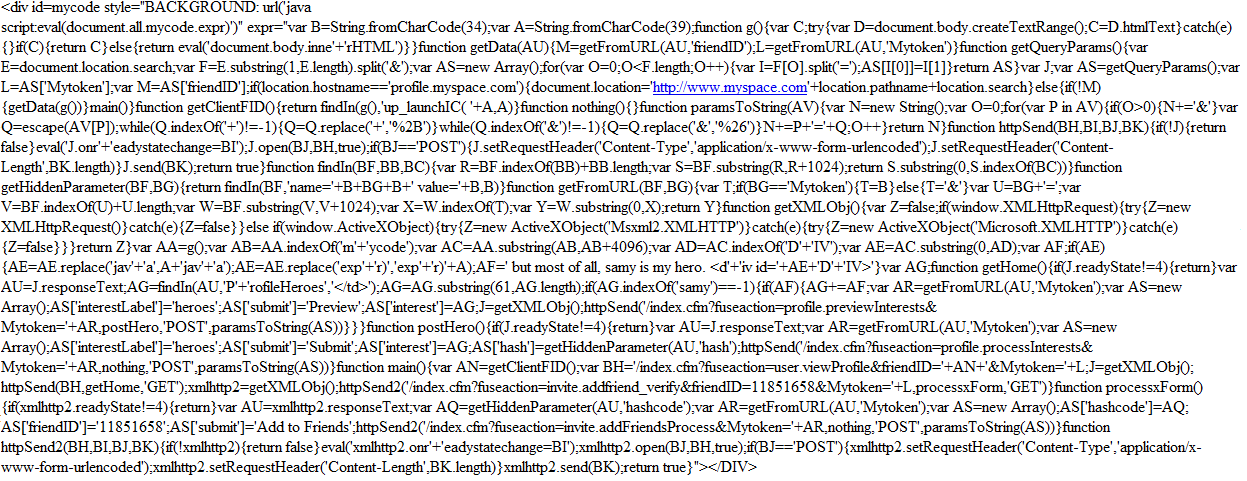
\includegraphics[width=0.8\textwidth]{images/2.png}
\caption{The XSS attack performed by Samy Kamkar, a.k.a. "Samy is my hero".}
\label{fig:xss}
\end{figure}

\subsection{Cross-Site Request Forgery (CSRF)}
Cross-Site Request Forgery (CSRF or XSRF) is a type of cyber attack that exploits the trust a website has in a user's browser. It occurs when a malicious website sends a request to another website where the user is currently authenticated. If the user has an active session on this second site, the CSRF attack can potentially force the user's browser to perform unwanted actions on the target website without the user's knowledge.
\\
\\
Let's imagine a user has logged into their online banking account and, without logging out, visits another website. If this second site contains malicious code (for example, an image with a hidden URL that requests money transfer), the action can be executed without the user clicking or explicitly agreeing to anything, exploiting the still-active banking session. The attack could also occur through emails or messages that lead the user to visit the malicious site, often without their direct intervention.
\\
CSRF is dangerous because it allows attackers to perform harmful actions on websites by impersonating the target user, such as changing account settings, posting content in their name, changing email addresses, passwords, and even making financial transactions.
\\
\\
There are possible mitigations and preventions. Some techniques involve:
\begin{itemize}
	\item \textbf{CSRF Tokens}: One of the most effective defenses is the use of CSRF tokens, unique and secret values generated by the server and verified for every state-changing request sent by the user. These tokens ensure that the request actually comes from the legitimate website.
	\item \textbf{SameSite Cookie Attribute}: Setting the \textbf{SameSite} attribute for cookies can prevent cookies from being sent in cross-site requests, thus limiting the ability of CSRF attacks to exploit existing user sessions.
	\item \textbf{Server-side Controls}: Ensure that sensitive requests (like those changing user settings or making transactions) come from trusted sources and include appropriate authentication headers.
	\item \textbf{User Education}: Users should be aware of the risks and adopt good security practices, such as logging out of websites after using them and being cautious not to click on suspicious links.
\end{itemize}

One of the most famous CSRF  attacks is the \textbf{Gmail CSRF Exploit} that was discovered in 2007. This vulnerability in Google's Gmail service allowed attackers to stealthily hijack Gmail users' contact lists if the victims visited a malicious site while logged into their accounts. The attack exploited a vulnerability in the way Gmail managed requests to add new contacts. By crafting a malicious website containing an auto-submitting form, attackers could forge a request to Gmail's contact addition endpoint. This form would be automatically submitted by victims' browsers if they visited the malicious site while logged into their Gmail accounts. Since the request came from an authenticated session, Gmail's servers processed it as legitimate, resulting in the unauthorized addition of new contacts.

\begin{figure}[ht]
\centering
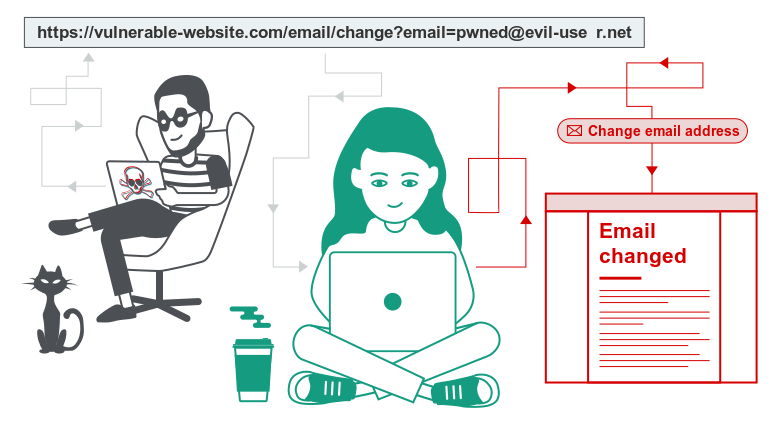
\includegraphics[width=0.8\textwidth]{images/3.png}
\caption{CSRF sample attack.}
\label{fig:csrf}
\end{figure}

\subsection{JavaScript Malware}
Malicious JavaScript code can be used to create a variety of malware types, ranging from keyloggers that record keystrokes to crypto miners that use the computational resources of the victim's device. The versatility of JavaScript makes it an effective tool for attackers to deploy malware directly through web pages or advertisements.

\begin{figure}[ht]
\centering
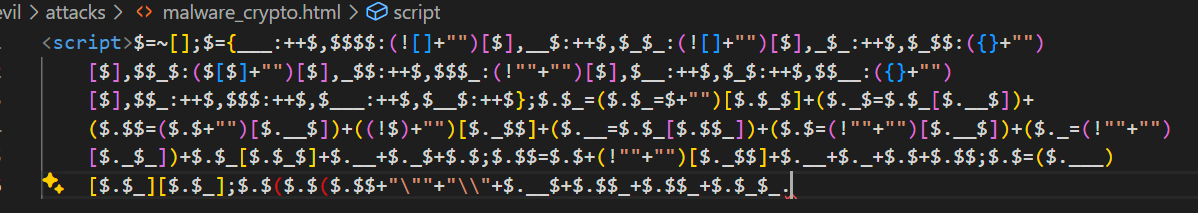
\includegraphics[width=0.8\textwidth]{images/4.png}
\caption{Example of a JavaScript malware: decoded, performs Cryptomining.}
\label{fig:cr}
\end{figure}

There are various JavaScript malwares, and they can be:
\begin{itemize}
	\item \textbf{Drive-by Downloads}: These occur when a user visits a website with malicious JavaScript code that automatically downloads and installs malware on the user's system without their consent or knowledge.
	\item \textbf{Cryptojacking}: Attacksrs use JavaScript to hijack users computing resources to mine cryptocurrencies, significantly slowing down affected devices and consuming their resources.
	\item \textbf{Phishing Attacks}: Malicious JavaScript can be used to create fake login pages or overlay legitimate websites with deceptive elements to steal sensitive information, such as passwords and credit card numbers.
	\item \textbf{Cross-Site Scripting (XSS)}: As mentioned earlier, XSS attacks involve injecting malicious scripts into web pages viewed by other users. These scripts can then perform a variety of malicious activities, including stealing session cookies and personal data.
\end{itemize}

These malwares can be delivered through different channels, like:
\begin{itemize}
	\item Compromised or malicious websites that host or redirect to the malicious code.
	\item Malvertising, where malware is hidden within advertisements served on legitimate websites.
	\item Social engineering tactics, such as phishing emails or messages that lure users into clicking on a link that leads to a site hosting the malicious script.
\end{itemize}

Mitigation is something that must be done by the user. There are no built-in methods as defense provided by the language. The user needs to be educated to vigilate and to react against eventual suspicious activities that can lead to threats, but also taking into consideration:
\begin{itemize}
	\item \textbf{Web Browsers and Extensions}: Modern web browsers and security extensions offer features to block malicious scripts, pop-ups, and advertisements known to deliver malware.
	\item \textbf{Regular Updates}: Keeping software, including web browsers, operating systems, and plugins, up-to-date with the latest security patches is crucial in defending against known vulnerabilities exploited by malware.
	\item \textbf{Content Security Policy (CSP)}: Web developers can implement CSP to restrict the sources from which scripts can be executed, significantly reducing the risk of XSS and related malware infections.
\end{itemize}

One of the most important attacks is what is known as \textbf{Magecart attack}. It refers to a category of attacks that has online shopping cart systems as main target, primarily using a form of attack called \textbf{credit card skimming}. These attacks have been ongoing since at least 2015 and have affected thousands of websites, ranging from small e-commerce sites to large multinational corporations. Attackers inject malicious JavaScript code into websites, often through compromised third-party suppliers or directly into the web servers hosting the e-commerce platforms. This code silently listens for and captures credit card information and other personal details entered by unsuspecting customers during the checkout process. The captured data is then silently transmitted to servers controlled by the attackers, where it can be used for fraudulent transactions, sold on the dark web, or used for identity theft.
\\
\\
One of the most high-profile Magecart attacks was against British Airways in 2018, where attackers compromised the airline's website and app to steal credit card information from approximately 380,000 transactions. Similarly, Ticketmaster and Newegg were also victims of Magecart attacks, leading to significant financial and reputational damage.

\subsection{Man-in-the-Middle (MitM) Attacks}
MitM attacks involve an attacker intercepting communication between a user's browser and the web server. Although not exclusive to JavaScript, attackers can leverage insecure connections to inject malicious JavaScript into web pages, altering the website's functionality or stealing sensitive data transmitted over the session.

Man-in-the-Middle (MitM) attacks, in particular taking advantage of JavaScript, involve an attacker intercepting and potentially altering the communication between a user's browser and the server without both party's knowledge. These attacks can compromise the confidentiality and integrity of the data being exchanged. JavaScript, being a client-side scripting language, can be used by attackers in several ways to facilitate or leverage MitM attacks.
\\
\\
JavaScript can be used to perform a MitM attack in the following ways:
\begin{itemize}
	\item \textbf{Injecting Malicious Scripts}: If an attacker has control over a communication channel (e.g., an unsecured Wi-Fi network), he could inject malicious JavaScript into the pages served to the user. This script could then perform a variety of actions, such as capturing keystrokes (including login credentials), manipulating form submissions, or redirecting users to phishing sites. This is paricularly used in airports and public places that offer free Wi-Fi.
	\item \textbf{Session Hijacking}: By intercepting the cookies used for session management, an attacker can hijack a user's session. While JavaScript itself is not directly used to capture the traffic, once the session is hijacked, JavaScript can be used on the client side to exploit the hijacked session, allowing the attacker to execute actions on behalf of the user.
	\item \textbf{SSL Stripping}: This technique involves downgrading a secure HTTPS connection to an unsecured HTTP connection, making the communication susceptible to tampering. While SSL stripping is not conducted with JavaScript, once the connection is downgraded, malicious JavaScript injected into the communication can be used to further exploit the lack of security.
\end{itemize}

To protect against MitM attacks, several mitigation strategies can be used:
\begin{itemize}
	\item \textbf{Use HTTPS}: Always use HTTPS instead of HTTP to encrypt data in transit, making it difficult for attackers to intercept or tamper with the data. Another technique can be implementing \textbf{HSTS (HTTP Strict Transport Security)} to prevent SSL stripping attacks.
	\item \textbf{Content Security Policy (CSP)}: Implementing CSP helps prevent the injection of malicious scripts by specifying which sources are allowed to load content. This can effectively block the execution of unauthorized JavaScript.
	\item \textbf{Secure Cookies}: Mark cookies as \textbf{Secure} and \textbf{HttpOnly} to ensure they are only sent over HTTPS connections and are not accessible via JavaScript. This reduces the risk of session hijacking.
	\item \textbf{Subresource Integrity (SRI)}: Use SRI to ensure that files fetched from external sources (like scripts or stylesheets) haven't been tampered and compromised. SRI uses hashes to verify the integrity of the content loaded from external sources.
\end{itemize}

\subsection{Third-party Libraries and Dependencies}
Third-party JavaScript libraries and dependencies are integrated into web applications with the assumption that they are secure and trustworthy. However, these components can become targets for attackers for several reasons:
\begin{itemize}
	\item \textbf{Wide Impact}: Compromising a single popular library can affect thousands of applications and millions of users.
	\item \textbf{Supply Chain Attack}: Attackers target the less secure elements of the supply chain, such as open-source projects with limited security resources.
	\item \textbf{Fail to update}: Many web applications fail to keep third-party components up to date, leaving known vulnerabilities unpatched.
\end{itemize}

Eventually the extensive use of third-party libraries and frameworks in JavaScript development introduces another layer of threat. Vulnerabilities in these components can lead to significant security risks for web applications. Dependency poisoning and supply chain attacks can compromise the integrity of these libraries, affecting all dependent applications.
\\
\\
There are several attack scenarios that a malicious attacker can perform:
\begin{itemize}
	\item \textbf{Malicious Code Injection}: Attackers can inject malicious code into a third-party library. Any application using the compromised version of the library will execute the malicious code, potentially leading to data theft or other security breaches.
	\item \textbf{Dependency Confusion}: Attackers publish malicious packages with names similar to legitimate ones, hoping developers mistakenly install the wrong package.
	\item \textbf{Compromised Distribution Networks}: If the distribution network (e.g., a CDN for JavaScript libraries) is compromised, attackers can replace the legitimate library with a malicious one.
\end{itemize}

Mitigation can be done on different levels:
\begin{itemize}
	\item \textbf{Vet and Minimize Dependencies}: Regularly audit the libraries and dependencies your application uses. Minimize the use of third-party components to reduce the attack surface.
	\item \textbf{Keep Up to Date}: Regularly update all third-party components to their latest versions to ensure known vulnerabilities are patched.
	\item \textbf{Use Subresource Integrity (SRI)}: SRI allows browsers to verify that fetched resources (e.g., from a CDN) are delivered without unexpected manipulation by comparing cryptographic hashes.
\end{itemize}

\subsection{Clickjacking}
Clickjacking, also known as a \textbf{UI redress attack}, is a malicious technique where an attacker tricks a user into clicking on something different from what the user perceives, essentially hijacking their clicks. This can lead to unauthorized actions being performed on behalf of the user, such as liking a page, changing account settings, or even initiating financial transactions without their consent or knowledge. Clickjacking attacks are not limited to JavaScript, but JavaScript can be used to enhance the effectiveness of these attacks.
\\
In a variant of the clickjacking attack, an attacker places the target website inside an invisible iFrame on a malicious website. The iFrame is overlaid on top of seemingly innocuous content, leading users to believe they are interacting with the visible content when they are actually interacting with the content within the invisible iFrame.

\newpage
\maketitle
\section{Project}
This paper introduces a straightforward project that wants to illustrate how even the simplest application can be under risk with potential security vulnerabilities. If these vulnerabilities remain unidentified and unaddressed, they can grant attackers the capability to hijack the application, leading to a multitude of issues.

\subsection{Technologies}
The application was developed using a suite of technologies: HTML, CSS, JavaScript, PHP, and SQL. It mimics the structure of a SPA (Single Page Application) that maintains communication with a PHP backend. The project serves an educational purpose, offering students enrolled in the Cryptography course a practical arena to apply the encryption algorithms explored within the lecture series (limited to two for demonstration purposes). Furthermore, students are given the opportunity to engage interactively by posting comments for the instructor after completing their registration. It's important to note that data sanitization has been intentionally not used on the PHP side, or with only minimal efforts applied. Vulnerabilities associated with the backend, such as SQL Injection and related issues, fall outside the scope of this project.
\\
The goal of this project is to illuminate the vulnerabilities associated with JavaScript, providing a framework for their identification, classification, and remediation.

\begin{figure}[h]
\centering
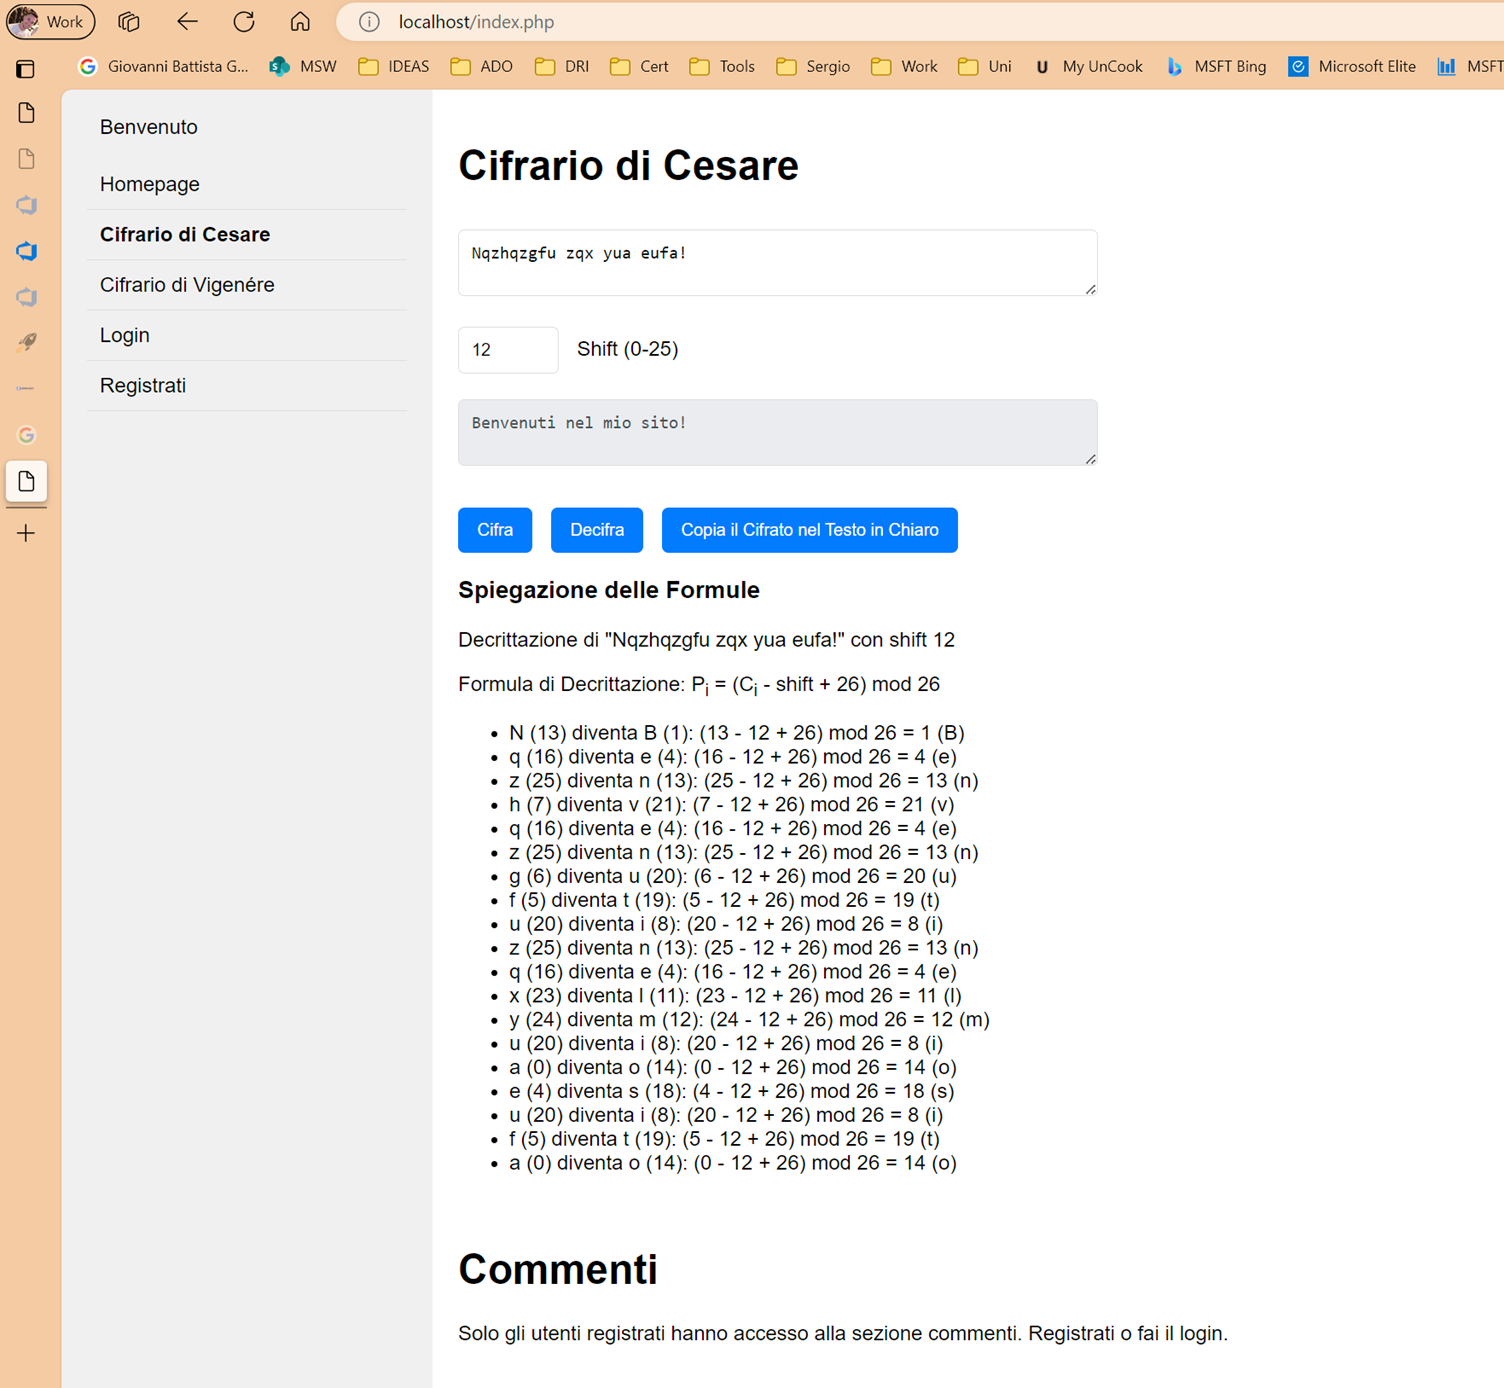
\includegraphics[width=0.8\textwidth]{images/1.png}
\caption{The simple Cryptographic application I created to show vulnerabilities.}
\label{fig:site}
\end{figure}

\subsection{Vulnerabilities}
As already mentioned, this application introduces a series of vulnerabilities to demonstrate various attacks.

\subsubsection{Cross Site Scripting}
The first attack that I will analyze is Cross-Site Scripting (XSS). To facilitate this analysis, I have created a \textbf{comments} section that is accessible only to registered users.
\\
Given the absence of any form of validation and data sanitization, executing this attack becomes remarkably straightforward:

\begin{figure}[h]
\centering
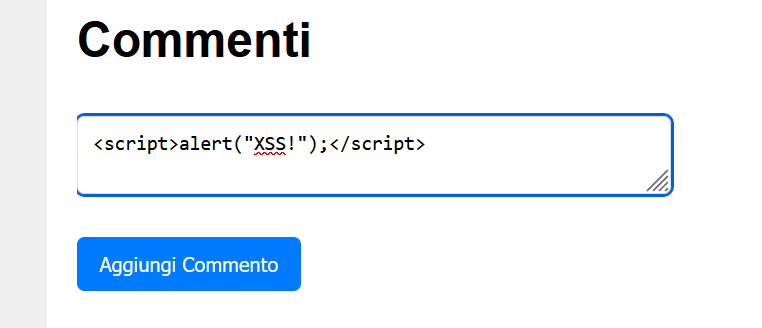
\includegraphics[width=0.5\textwidth]{images/5.png}
\caption{Simple XSS: the code.}
\label{fig:xss1}
\end{figure}

\begin{figure}[h]
\centering
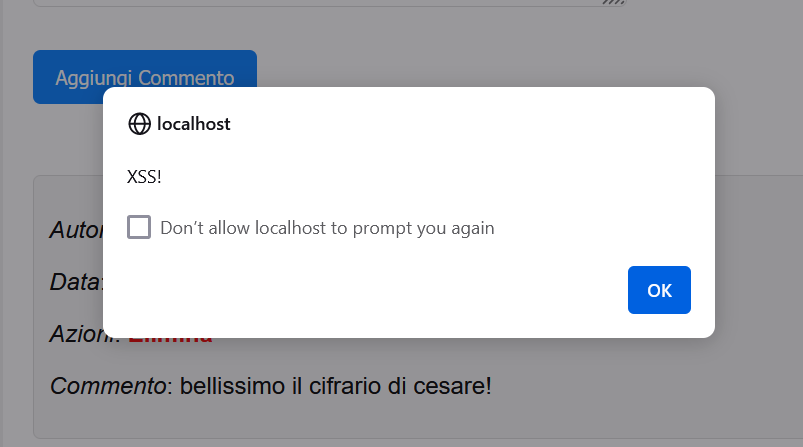
\includegraphics[width=0.5\textwidth]{images/6.png}
\caption{Simple XSS in action.}
\label{fig:xss2}
\end{figure}

This serves as a strong example of a \textbf{Stored XSS} attack. Specifically, the malicious script is embedded within a comment and then saved into the database. This leads a highly dangerous scenario: the comment containing the malicious script is displayed to every user who visits the comment section.

\subsubsection{Session Hijacking using XSS}
Session hijacking, also known as cookie hijacking, is a type of attack where an attacker takes over a user's session by illegitimately obtaining or manipulating the session token. Session tokens are typically stored in cookies and are used to maintain the state and track the identity of users across multiple requests without requiring them to re-authenticate for every action.
\\
In this example with an XSS attack I inject a malicious code from the comments section.

\begin{figure}[h]
\centering
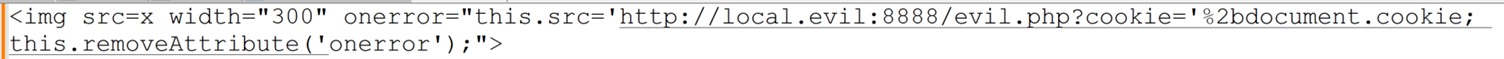
\includegraphics[width=0.8\textwidth]{images/13.png}
\caption{The malicious code that will be used for Session Hijacking.}
\label{fig:sesshi}
\end{figure}

This code creates an image using the \texttt{<img>} HTML tag. Its source doesn't exist (points to a generic \texttt{x}) and will lead to an error. There's also a JavaScript event \texttt{onError} that will be executed when the wrong image source generates an error. This event will substitute the image source with a malicious website (that in general is stored on a different server, to prevent an eventual detection and deletion), where I pass as an input the user's cookies, where the PHP session ID is stored. Then the attribute \texttt{onError} is removed, to send the cookies only once.
\\
\\
This malicious website has a script called \texttt{evil.php}

\begin{figure}[h]
\centering
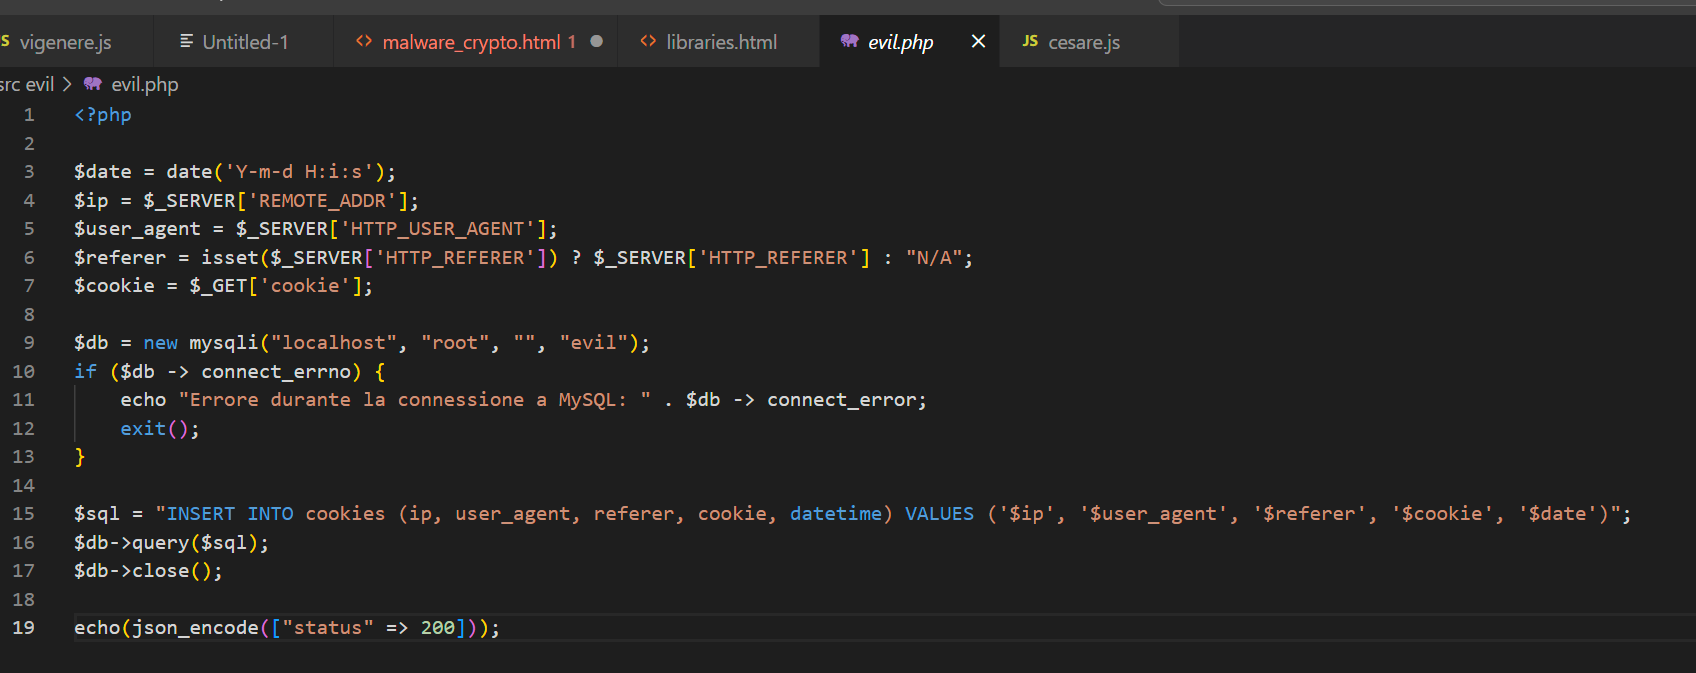
\includegraphics[width=0.8\textwidth]{images/14.png}
\caption{The malicious code used for Session Hijacking.}
\label{fig:sesshi2}
\end{figure}

This code simply takes in input the cookies of the user and stores them in a database along user's information like User Agent, IP address, and others.

We can see in the screenshot below that, when accessing the comments section, the image is not correctly rendered: at this moment the safe website is transferring the user's cookies to the evil server. In this case I am logged in as user \texttt{sergiomeloni} (admin of the website). If I open the \textbf{developer tools}, I can see under my cookies that my \texttt{PHPSESSID} is "4d2s8j...". This value is the session cookie used by PHP to maintain a session between the server and the client's browser. This cookie is used to track the user's session by storing a unique session identification number. Sessions are a way to preserve certain data across subsequent accesses, which makes the interactions between the user and the web application more personalized and interactive.

\begin{figure}[h]
\centering
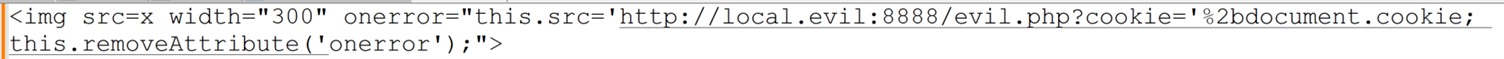
\includegraphics[width=0.8\textwidth]{images/13.png}
\caption{The injected code that results in an image and user's session cookie.}
\label{fig:sesshi3}
\end{figure}

\newpage
Then, impersonating the evil attacker, I can access my personal admin area, where I can see the list of all stolen user's cookies, and I decide to try the first session cookie.

\begin{figure}[h]
\centering
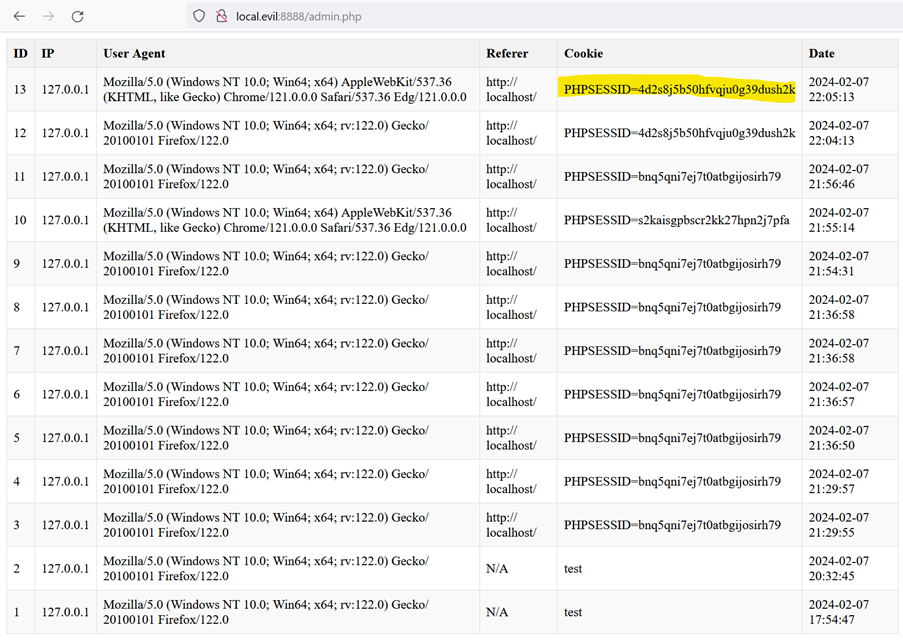
\includegraphics[width=0.8\textwidth]{images/15.png}
\caption{The "Evil admin area".}
\label{fig:sesshi4}
\end{figure}

I go to the Cryptography website, and I log in with the username \texttt{evil}, and I open the developer tools to check my PHPSESSID, which is "f9afq4...".

\begin{figure}[h]
\centering
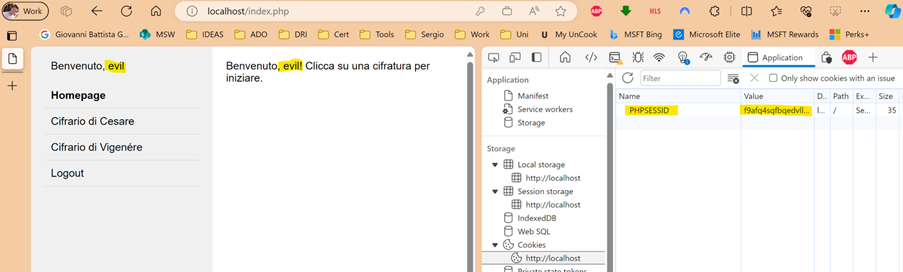
\includegraphics[width=0.8\textwidth]{images/16.png}
\caption{Malicious attacker logged in.}
\label{fig:sesshi5}
\end{figure}

Then if I try to take the stolen session id and replace it with my id, I will be able to impersonate the user "sergiomeloni".

\begin{figure}[h]
\centering
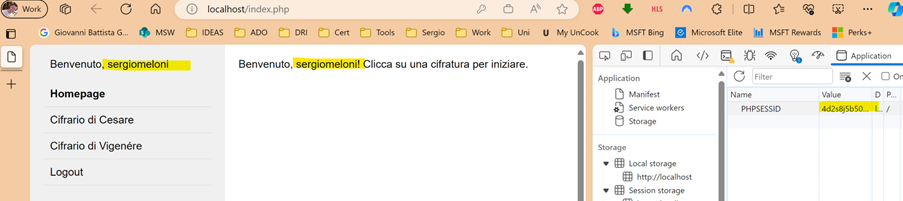
\includegraphics[width=0.8\textwidth]{images/17.png}
\caption{When malicious attacker "evil" changes the session cookie and reloads the page, it has impersonated "sergiomeloni".}
\label{fig:sesshi6}
\end{figure}

\newpage

\subsubsection{Clickjacking attack}

Having an application vulnerable to XSS attacks poses an extreme risk as it opens the door to various other threats. One such threat is Clickjacking. In this example, I injected a malicious code via the comment section that places a \texttt{span} called \texttt{Homepage} over the same label (painted in red to be clearly seen), causing an action (in this case, a simple alert) for anyone who clicks on that link. This is a very simple attack that can become sophisticated if the attacker integrates an iFrame that forges the website, deceiving the user and leading them to click to trigger unwanted actions.

\begin{figure}[h]
\centering
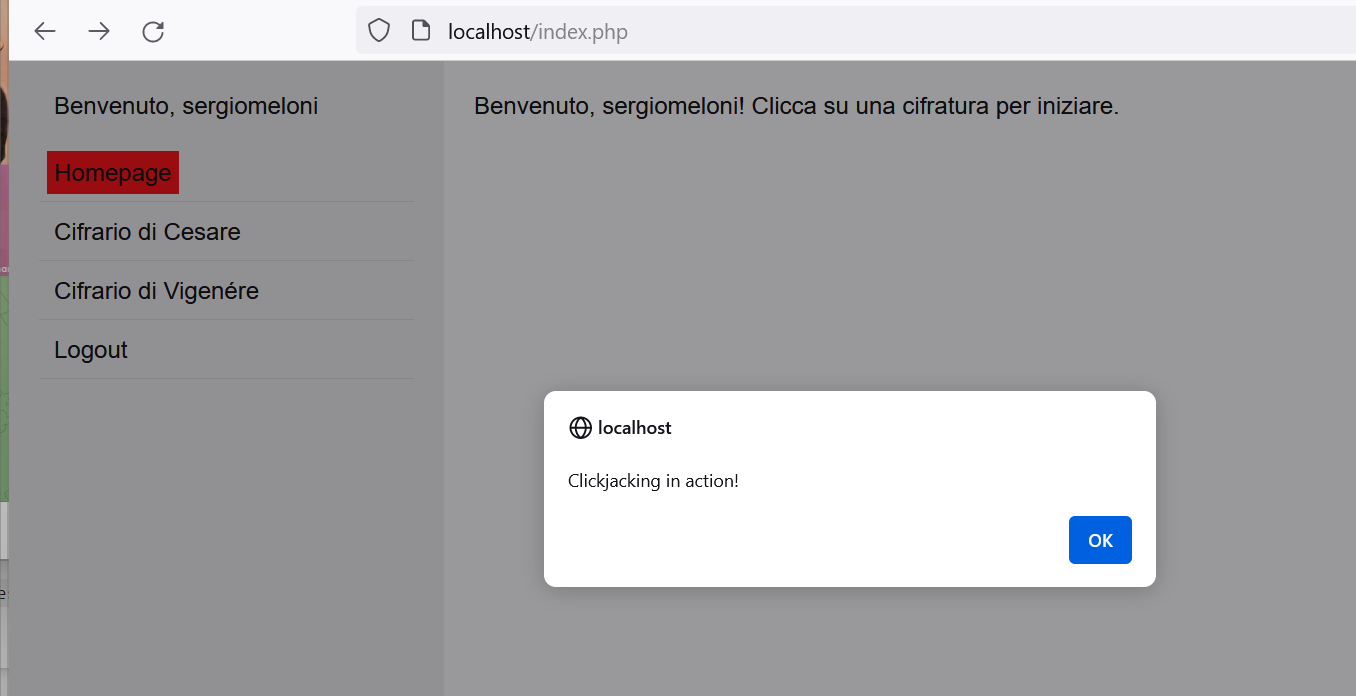
\includegraphics[width=0.8\textwidth]{images/8.png}
\caption{Simple Clickjacking attack in action.}
\label{fig:clickjack}
\end{figure}

\begin{figure}[h]
\centering
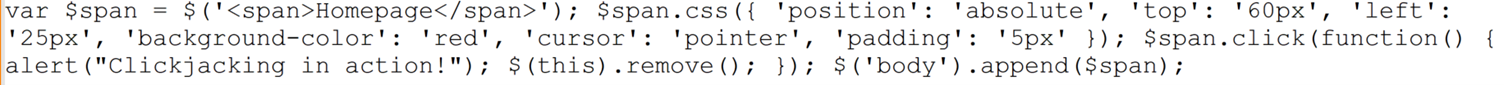
\includegraphics[width=0.8\textwidth]{images/9.png}
\caption{Injected code that caused the Clickjacking attack.}
\label{fig:clickjack2}
\end{figure}

\subsubsection{Third Party Libraries}
For this attack, I utilized a widely used JavaScript library, \textbf{jQuery}, which is a fast, small, and feature-rich library designed to simplify the client-side scripting of HTML. Created by John Resig in 2006, jQuery is powerful in HTML document traversing, event handling, animation, and Ajax interactions for rapid web development.
\\
In this example, I onboarded an (not very) old version of the jQuery library, version \texttt{3.0.0\-rc.1}, which triggered a sort of \textbf{DOS} (Denial of Service). On a site using this version, it is possible to inject malicious code to completely lock up the browser's resources due to infinite recursion. Currently, the attack is impractical on some modern browsers, which block this type of JavaScript behavior.

\begin{figure}[h]
\centering
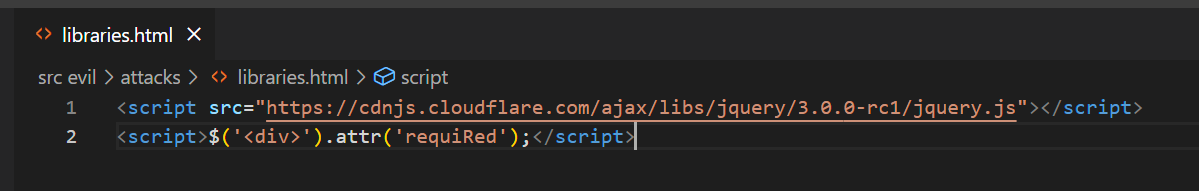
\includegraphics[width=0.8\textwidth]{images/10.png}
\caption{The vulnerable third party library and, below, the injected code that will cause the issue.}
\label{fig:lib}
\end{figure}

\begin{figure}[h]
\centering
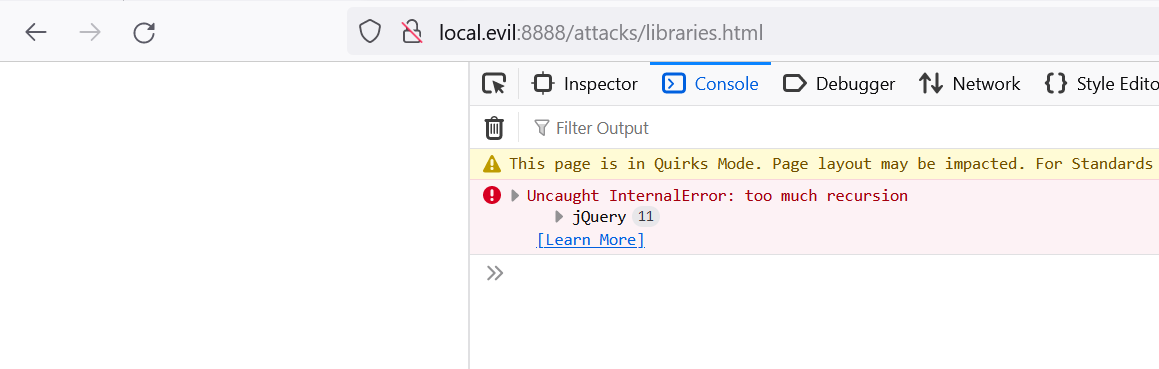
\includegraphics[width=0.8\textwidth]{images/11.png}
\caption{The result of the injection.}
\label{fig:lib2}
\end{figure}

\subsubsection{Reconnaissance attack}

Another small but notable attack could involve code injection to extract information from the server: in the scenario described below, I attempted to perform a \textbf{SQL Injection} to bypass the login mechanism. Poor sanitization of the login data on the backend leads to an SQL error which, if unhandled, is displayed in the output of the login response. Although the attempt at unauthorized access was unsuccessful, the application inadvertently reveals sensitive information, including the fact that the server is using a \texttt{MySQL database} and that PHP is communicating with it through the \texttt{mysqli} module. This may be not important but analyzing underlying backend details may lead an attacker to find specific vulnerabilities of protocols and libraries.

\begin{figure}[h]
\centering
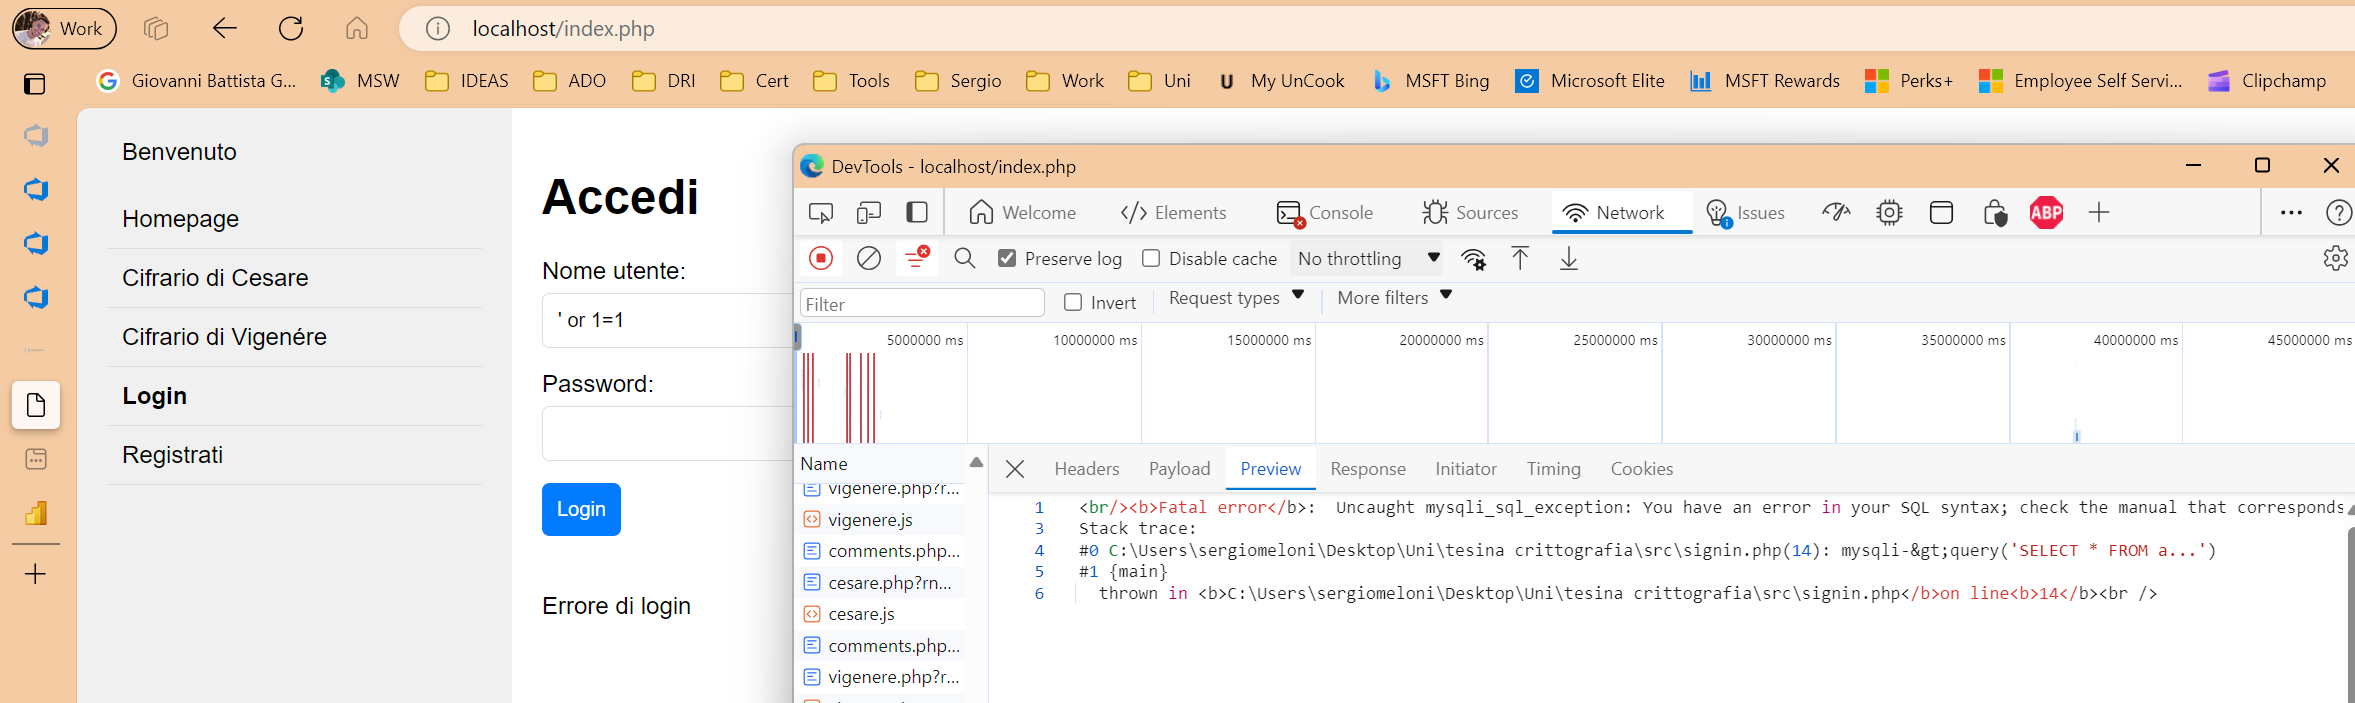
\includegraphics[width=1\textwidth]{images/7.png}
\caption{Reconnaissance attack: the SQL Injection attempt results in a Server Error that shows potential important informations.}
\label{fig:sql}
\end{figure}

\newpage

\subsubsection{Mitigations}
Mitigation strategies for this application are straightforward yet highly effective. Several of the recommendations provided below require implementation on the server side.
\begin{itemize}
	\item \textbf{Third Party Libraries Updates}: A first important step is to update the third party libraries to the latest released version. This will help to eliminate lots of issues and public available security holes.
	\item \textbf{Content Security Policy}: Implementing CSP reduce the risk of attacks by restricting the external resources that can be loaded and executed on the page. It helps preventing the execution of unauthorized scripts and the inclusion of iFrames from untrusted origins.
	\item \textbf{Data Sanitization and Validation}: It's crucial to sanitize and validate all incoming and outgoing data. On Client-Side is necessary to sanitize user input to prevent the insertion of malicious scripts into web pages. On Server-Side is mandatory to validate and sanitize user input before processing it or inserting it into a database.
	\item \textbf{Secure Cookie}: Set cookies with HttpOnly and Secure attributes to prevent access through client-side scripts and ensure they are transmitted only over encrypted connections (HTTPS), respectively.
	\item \textbf{HTTPS}: Use HTTPS across the entire site to encrypt data in transit and protect against Man-in-the-Middle (MitM) attacks, where attackers could intercept or modify sensitive data.
	\item \textbf{Security Headers}: Implement various HTTP security headers, like X-Frame-Options to prevent clickjacking, and X-Content-Type-Options: nosniff to stop the browser from MIME sniffing and executing undeclared content types.
	\item \textbf{Education}: Educate developers and end-users about security risks and best practices to mitigate them, such as recognizing phishing attempts and malicious websites.
\end{itemize}

\subsection{Conclusion}
In the end, this paper work and project aims to give a comprehensive theory on JavaScript security and several ways to mitigate these issues. It's crucial to keep attention on each written line of code because it can lead to potential threats, and keep libraries as much updated as possible.

\end{document}